\chapter{Urban Land and Land Rent} \label{chapter-space}
\epigraph{Where are intellectual spillovers more obvious than in dense, urban environments?}{Edward L. Glaeser,\cite{glaeserCitiesInformationEconomic1994} Cities, Information, and Economic Growth, 1994}
\epigraph{One of the very important components in the urban and agricultural land use model is the so-called \gls{bid-rent curve}. Regional and urban economists, city planners, and economic geographers have used this curve extensively as an analytical device.}{\cite{shiehWilhelmLaunhardtBidRent2004}}

The goal of this chapter is to describe informally the urban model that serves as a bridge from the growth theory we use to urban space and rent distribution.  Although the model is easily generalized, we restrict our presentation to the highly  stylized core version to establish how land rents are generated in the urban system and how they are related to neoclassical growth theory. The feature of the model that provides the necessary link is known as the `\gls{bid-rent curve}.' We will go on in Chapter~\ref{chapter-financialization} to incorporate  the  financial sector into  land market  curve via the bid-rent.



\section{The Alonzo-Jacobs model}

We will refer to the core urban model developed by Alonso \cite{alonsoLocationLandUse1964}, Muth \cite{muthCitiesHousingSpatial1969} and Mills \cite{millsAggregativeModelResource1967}, and later formalised by Wheaton \cite{wheatonComparativeStaticAnalysis1974} and others, as the ``Alonzo Model.''\footnote{it is also called the Alonzo model, the Alonzo-Muth model, the Alonzo-Muth-Mills model, the circular city model, and the monocentric city model.} William Alonso published \textbf{Location and Land Use} in 1964  \cite{alonsoLocationLandUse1964} based on his 1960 Phd thesis,\cite{alonsoModelUrbanLand1960} 
giving him a slender priority in the literature.  Richard Muth's \cite{muthSpatialStructureHousing1961}, and \cite{muthRationalExpectationsTheory1961},  were written roughly simultaneously with and independently of Alonso's thesis, and  culminated in Muth's classic book, Cities and Housing  \cite{muthCitiesHousingSpatial1969}.\footnote{See ``William Alonzo, Richard Muth, Resources for  the Future, and the founding of urban economics''\cite{mcdonaldWilliamAlonsoRichard2007} for a more detailed discussion of the development of the model.}   It is worth noting that Lowdon Wingo also had a manuscript of  ``Transportation and Urban Land'' \cite{wingoTransportationUrbanLand1961}(1961)  in preparation that presented a core idea and  significantly influenced Muth \cite{mcdonaldWilliamAlonsoRichard2007}. Mills' ``Urban economics'' \cite{millsUrbanEconomics1972} followed soon after. The early 1960s were a watershed in urban economics, and the model rapidly became the workhorse for theorists and empirical researchers.

 The seeds of the bid-rent curve at the heart of the model were presented as early as 1885  by German engineer-economist Wilhelm Launhardt. \cite{blaugEconomicTheoryRetrospect1985, launhardtMathematischeBegruendungVolkswirthschaftslehre1885} The  \gls{bid-rent function} was first applied explicitly to the equilibrium of land use patterns in agricultural production by August Losch \cite{loschEconomicsLocation1954} in Germany and Edgar S. Dunn \cite{dunnEquilibriumLandUsePatterns1954} in America, and was later extended to the urban setting by William Alonso \cite{alonsoModelUrbanLand1960}. Alonzo's  model  specifically linked the urban wage premium to urban land rents through transportation costs.  Bruckner \cite{bruecknerStructureUrbanEquilibria1987} describes it as ``a simple yet powerful model of urban spatial structure that successfully explains the principal regularities observed in the urban landscape,'' and goes on to say, ``the good predictive performance of the model suggests that its simplifications are artfully chosen, capturing the essential features of real-world cities''. It rapidly  became the central model in modern urban economics.

The Alonzo model, long  recognized as a persistent law in urban and regional studies, is actually a model of competitive real estate markets: in less than competitive markets, other factors may affect bid rents significantly.
Gao et al \cite{GaoJinlong2020BtbT}, for example,  found  that for China, ``other  exogenous  factors –– including  the  distinct  land  system  and  centralized  political  institutions -- also matter a great deal''. In general, however, 
research has largely supported the bid rent model (\cite{mutoEstimationBidRent2006, wheatonBidRentApproach1977}) Muto \cite{mutoEstimationBidRent2006}, for example concluded that,  ``land usage on average follows the rule that is consistent with the bid rent function model: whichever usage outbids the others occupies the land. ''  Borba1 and Dentinhoand \cite{borbaEvaluationUrbanScenarios2016} concluded that ``The method has proved its usefulness and effectiveness for predicting the impacts of exogenous shocks in complex urban systems.'' 
%
In a test for the city of Bogota, Gross \cite{grossEstimatingWillingnessPay1988} found that  ``the bid-rent model works reasonably well in its predictions and in its estimates of the demand for attributes and, in some ways, it may perform better than a hedonic-type model in forecasting the demand for housing attributes.'' 
%
Clay and Valdez incorporate bid rent model into an integrated ABM transportation-land use mode that achieves levels of accuracy similar to the best models currently available. These are the microsimulation of UrbanSim\footnote{UrbanSim is a microsimulation land use model, designed to support the need of Metropolitan Planning Organizations (MPOs), cities and other organizations for analyzing the potential effects of land use policies and infrastructure investments on the development and character of cities and regions. The core model code has been developed in the Python programming language as Open Source software and is publicly available on the Urban Data Science Toolkit GitHub page.\cite{waddellmodellinurbandev2002}}; and the bid-rent submodule of \footnote{PECAS is  HBA Specto Incorporated's commercial modelling system  for simulating spatial economic systems.} developed by Abraham and Hunt (2005). the best models currently available. They emphasisze the advantage of ABM model is allowing for agents to differ in composition and in preferences making them unique bidders. 
% Agents must compute the maximum bid price they are willing to pay.
An earlier analysis by Curran and Carlson \cite{curranTheoryResidentialLocation1982}, among other, extended the bid-rent model include two-worker households and a secondary employment location. They showed that households whoudl bve expected to segregate spatially, but the pattern will depend on the specific combination of wages, transport costs and the mix of household types in the populations. 
Because our goal  is to extend current model by introduce speculative motives and financialization, we retain the single-type household of the basic model, we defer the  question of the differential effect on household types for later work.  
%

We use what we choose to call an \textbf{Alonzo-Jacobs} version of the model to explore the source and distribution surplus value. The reference to  the agglomeration effects that Jane Jacobs  described in her great book, The Economy of Cities \cite{jacobsEconomyCities1969}. an that generate the  \gls{urban wage premium} central to urban growth. % and the wage premium. 

To situate the model further, recall that Ricardo had described a model with a central market for corn, producing corn took land and transporting corn to market was costly. Because there is one market price for corn, land with low transportation costs near the central market earns a rent.\footnote{In most of the discussion Ricardo emphasized  differential land fertility rather than distance to market.} More distant land has lower value. In Alonzo's model there is central market and a single price for labour, producing labour takes land, and transporting labour to the market is costly. Alonzo re-presents Ricardo's conception of rent  mathematically for a different social system and production technology.  

The logic of the model is illustrated in Figure~\ref{fig-alonzo-simple} for a city on a uniform plane with a population of identical workers who work at the city centre, have identical housing needs,  identical transportation costs and receive the same wage. Transportation to and from the center costs ${c}$ times the distance $d$ from the center. Fuel, capital, and time costs are  all included in $t$. The figure represents housing value and transportation cost at every point along the thin slice of the city from the centre to its edge at $d^*$.  It is common to assume that the labour market and production sector at the centre take no space. 

 Since individuals would simply move to any location that offered a higher utility, in an equilibrium all the otherwise identical workers must receive the same utility. This has to be the case even though those farther from the center must pay more for transportation to and from home. The variable that  adjusts to maintain equal utility with rising transportation spending is the cost of housing. Thiis conception of a locational equilibrium is the heart of the model and all its extensions.

The height of the green bar on the left illustrates the wage premium for urban labour at the centre of the  city. 
The height red triangle adjacent the green bar represents the amount of rent earned on land at the centre, which has no transportation costs. The entire red triangle is aggregate land rent generated by the city along the slice.\footnote{The model says nothing about who gets the rent in the urban economy. For classical economists it was obvious that the agricultural rents went to the class of land-owners.} Transportation to and from the center costs $t$ times the distance $d$ from the center. Fuel, capital, and time costs are  all included in $t$. 

% %%%%%%%%%%%% PARTITIONING THE LABOUR SHARE
\begin{figure}
    \begin{center}
    
% Simple Alonzo model
%%%%%%%%%%%%%%%%%%%%%%%% PARTITIONING THE LABOUR SHARE
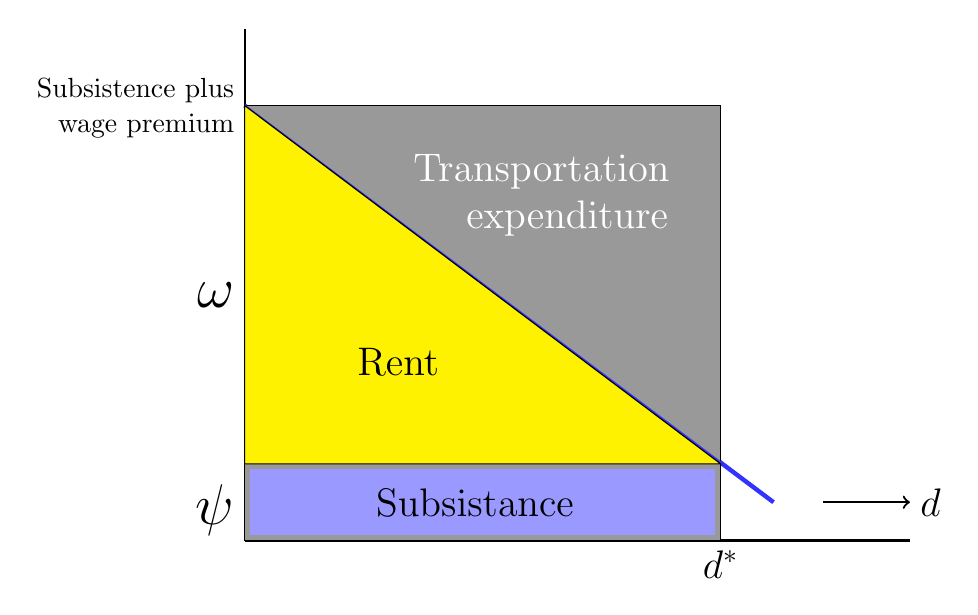
\begin{tikzpicture}[scale=.65]
\def\bndmax{5}        %https://tex.stackexchange.com/questions/68462/filling-a-complex-region-with-tikz
\def\bndmin{0.2}
\def \n {8.5}  % height of y axis
\def \d {13}  % length  of x axis
\def \t {.75}  %  cost of transportation per unit x
\def \th {1}   %
\def \w {7}    %  wage premium
\def \om{1.5}%  omega =rural wage Zero for urban population
\def \azero{2}
\def \aprime {-.0}	
\tikzset{func/.style={thick,color=blue!80}}	

% FIRST FIGURE just axes PARTITIONING THE LABOUR SHARE
\draw [thick] (0,-\om) --(\d,-\om);  			% Zero for rural population
\draw [thick] (0,-\om) --(0,\n); %node[above]{\Huge $w$};	% Y axis
%\node at (0,\n+0.5){\large $Rent$};

% \draw [thick] (0,0)node[left=.5]{Subsistence}--(\d,0);
%\node at(-2,1) {$\omega$};
\node[left=.25] at (0,3.3){\huge $\omega$};
\node[left=.25] at (0,-0.9){\huge $\psi$};
%\node[left=.25] at (0,3){$w+\omega$};
\node[left=.25] at (0,\w+.3){Subsistence plus};
\node[left=.25] at (0,\w-.4){wage premium};	

%\foreach \xi in {0,..., \n} \draw (\xi,0)--(\xi,-.1)node[below=1]{\small$\xi$};
%\foreach \yi in {1,...,\n} \draw (0,\yi)--(-.1,\yi)node[left]{$\yi$};
%\foreach \i in {1,4,9,16} {
%\node at (7,-\om/2){people scattered uniformly across the land  };

%SECOND FIGURE WITH AGGLOMERATION WAGE
%   \pause %  add urban production and net wage PARTITIONING THE LABOUR SHARE
%\draw[fill=white, white] (0.1,-0.1) rectangle (14,-\om+.1);
%\draw [fill=green!80] (-.25, 0) rectangle(.25, \w);
\node[right] at  (.25, \w/2){Added Productivity};
% \node[right, text width = 3cm] at  (10,9){Where does the increase in productivity come from?};
\draw [ thick, ->](11.3,-\om/2)--(13, -\om/2)node [right] {\Large $d$};

%  THIRD FIGURE  add wage profile PARTITIONING THE LABOUR SHARE
% \pause
%\node[right, white, fill=white,  text width = 3cm] at  (10,9){Where does the increase in productivity come from?};
\draw[func, domain=0:\w/\t+1,ultra thick] plot [samples=200] (\x,{\w-\t*\x}); %Net wageprofile  for 
%\node[right, white, fill=white] at  (.25, \w/2){Added Productivity};
%\node[right, fill=white, text width =3.5cm ] at  (1, \w/2){Declining wage  net \\of transportation\\ costs $T(d)$ };

%   FOURTH FIGURE     commuters PARTITIONING THE LABOUR SHARE
%\pause
%\draw[fill=blue!40] (0.1,-0.1) rectangle (9.2,-\om+.1);
%\node at (4.5,-\om/2){commuters};

%   FOURTH FIGURE    wage bill
%\pause %add total new value
\draw[fill=green!40] (0,-\om) rectangle(9.30,\w);% new product
\node at (4.5,\w/2){\Large urban wage bill};

%%   FIFTH FIGURE   distribution
%\pause
%\node at (9,\n){\Large Partitioning the Labour Share};

\draw[fill=black!40] (0,-\om) rectangle (9.30,\w);% new product repeat
\draw[func, domain=0:\w/\t+1] plot [samples=200] (\x,{\w-\t*\x}); %rent profile
\fill[blue!40] (0.1,-0.1) rectangle (9.2,-\om+.1);
\node at (4.5,-\om/2){\Large Subsistance};
\draw[fill=yellow,] (0.,0.) -- (0,7)--(9.30,0.)--cycle;% Rent \w-.2
\node at (3.,2){\Large Rent}; 		%Rent 
\node at (5.8,5.7)[white]{\Large Transportation};
\node at (6.3,4.8)[white]{\Large expenditure};
\node at (9.3,-1.5)[below]{\Large  $d^*$};
% \node at (4.8,\w)[above]{\huge $d^*$};
 \end{tikzpicture}
 

    \caption{}
    \label{fig-alonzo-simple}
    \end{center}
\end{figure}

The entire rectangle, $\omega$ $\times$ $d^*$, is the wage bill generated by urban agglomeration. Urban land rent is the residual when transport costs are deducted from the wage premium. It declines  with distance $d$ until, at the very edge of the city, $d^*$, the cost of transportation  consumes the entire wage ($td^*=\omega$). The grey triangle represents the amount of the surplus dissipated in travel costs.  Property values are simply the the present discounted value of the rent at any point.

At the bottom of the figure we illustrate the conventional `subsistence wage'  earned by a worker whether in the city or outside of the city.   In most analyses of urban spaces this living wage is simply ignored, since it is the wage premium that generates rents.  The relative size is unimportant because it is the same for urban and non-urban workers. If urban consumption is higher than non-urban consumption it must come out of the land rent.
%Workers are attracted to the city by the wage premium, $\omega$,  which represents the share of the surplus generated by the city that goes to labour.  
\footnote{If the city generates additional social amenities\index{amenities} not captured in the wage  the money available for housing does not change, although willingness to pay must be higher.  The  most likely adjustments are in urban `subsistence' and it is probably offset by rural amenity that is given up to live in the city. In the long run urban amenities must exert upward pressure on rural amenities. These interesting extension will not be taken up in this thesis. }

The extent  of the city  $d^*$ is a simply the distance at which total $rt$ transportation cost  is equal to the wage premium
\[d^* t= \omega\]
where $t$ is the unit cost of transportation. In the figure, $-t$ is the slope of the diagonal line dividing rent from transportation expenditure.



 \subsection{The magnitude of rents and transportation costs}
 From $w$, $t$ and population density we can derive population, wage bill, total rent, transportation costs. The figure above suggest that  half of the urban surplus is spent on transportation, but because the city is circular, the total value of rents can be represented as  a cone with the volume  \[ V=\frac{1}{3}\pi  d^{*2} \omega \]
of a cone with radius $d^*$ and  height $\omega = td^*$. Substituting out either  $\omega$ or  $d^*$, we find that total rent is  proportional to the \textbf{cube} of either  $d^*$ or $\omega$. 

The total value of wage payments appears as the volume of cylinder enclosing the cone\footnote{since the wage is the same for each unit of labour no matter where it resides.}.  
$V=\pi r^2 \omega$ 
and total transport costs are 
$\frac{2}{3}\pi  d^{*2} \omega).$
With uniform density, population is proportional to the square of  $d^{*2}$ while rents and  transportation costs are proportional to the cube. %move this?

\begin{figure}
    \begin{center}
    
\begin{tikzpicture}[scale=.5]
   %%%%%%%%%%%%%%%%%%%%%%%%%%%%%%%%%%%%%%%%%%%%%%%%
% definitions for schematic
\def\bndmax{5}        %https://tex.stackexchange.com/questions/68462/filling-a-complex-region-with-tikz
\def\bndmin{0.2}
\def \n {10}  % height of y axis
\def \d {12}  % length  of x axis
\def \t {.75}  %  cost of transportation per unit x
\def \th {1}   % theta?
\def \w {7}    %  wage premium
\def \om{1.5}%  omega =rural wage Zero for urban population
\def \azero{2}
\def \aprime {-.0}	
\tikzset{func/.style={thick,color=blue!90}}	

    %%%%%%%%%%%%%%%%%%%%%%%%%%%%%%%%%%%%%%%%%%%%%%%%
% definitions for Cone3
%\node at (0, 2.5){\input{SA_Cone3.tex}};
     \pgfmathsetmacro{\radiush}{9.7};%Cone base radius was 9.6
        \pgfmathsetmacro{\theight}{7.1}%Cone height (negative if you want a inverse cone)
        \pgfmathsetmacro{\cheightp}{.03}%Cut height in percent of cone height

        %Calculating coordinates
        \coordinate (center) at (0,0);
        \pgfmathsetmacro{\radiusv}{.2 * \radiush}; %HORIZONTAL RADIUS
        \coordinate (peak) at ($(center) + (0,\theight)$);     
        \pgfmathsetmacro{\sradiush}{\radiush * (1 - \cheightp)};%ADJUST FOR COVERAGE AT CORNERS
        \pgfmathsetmacro{\sradiusv}{.2 * \sradiush};
   %     \pgfmathsetmacro{\sradiusv} {\sradiusv -.1 };

\coordinate (antipeak) at ($(center) + (0,-\theight)$);  %thanks  %I added this
\coordinate (vert1) at ($(center)+(\radiush,-.2)$);
\coordinate (vert2) at ($(center)-(\radiush,.2)$);
%problem
   
\coordinate (svert1) at ($(vert1)!\cheightp!(peak) +(0.1,.75)$);
\coordinate (svert2) at ($(vert2)!\cheightp!(peak)+(.5,.75)$);  
    % \coordinate (svert3) at ($svert1+(0,\w)$);
    % \coordinate (svert4) at ($vert2)+(0,\w)$);  
    %  \coordinate (svert3) at ($svert1+(0,7)$ );  % Shifting up by W
    % \coordinate (svert4) at ($svert2 + (0,\w)$0;
   %%%%%%%%%%%%%%%%%%%%%%%%%%%%%%%%%%%%%%%%%%%%%%%%


 
%\draw[step=.5,black,thin] (-9.6,0) grid (9.6,7);
 
% Cone Drawing    
 \fill[ left color=red!70, right color=red!70,  opacity=20,middle color=red!20,shading=axis] (svert1) -- (peak) -- (svert2) arc (170:370:\sradiush cm and \sradiusv cm);

    % FAT GREEN BAR
 \draw [fill=green,opacity=80] (-.2, 0) rectangle(.2, \w);
 \node[above] at (0,\w){$\omega$};
 
%Uncomment this for top of cylinder
      \fill[inner color=gray!2,outer color=gray!40,shading=radial,opacity=.5] ($(center) + (.35,\theight)$ ) circle (9.4 cm and 1.55 cm );
      
        % \draw [thick]($(svert1) +(.3,-.3)$)-- ++ (90:\w-.2);
        % \draw [thick]($(svert2)-(.2,.3)$)-- ++ (90:\w-.2);
        %Lines, \h in percent of cone height
 def \sradiusv2 \sradiusv cm -.1 cm)
% Cylinder drawing
  \fill[ left color=black!50, right color=red!30,  middle color=red!30,shading=axis,opacity=.2]  (-9.05,.5) 
  arc (180:360:\sradiush cm and \sradiusv cm)-- ++(90:\w-.2) 
  arc (360:180:\sradiush cm and \sradiusv2 cm -.1 cm)--(-9.05,.5);  

   \node[above] at (0,\w){\Large $\omega$};
% TRY TO Make a cylinder
%\draw ($svert2 + (0,\theight)$) [arc (180:360:\sradiush cm and \sradiusv cm)]; 
%     \fill[left color=gray!70,right color=gray!70,middle color=gray!30,shading=axis] (vert1) -- (svert1) arc (0:-180:\sradiush cm and \sradiusv cm) -- (vert2) arc (180:360:\radiush cm and \radiusv cm);

% DASHED LINE AT BACK OF CONE
\foreach \h in {0.03}{   %.38,.34,.30, .7
            \pgfmathsetmacro{\rh}{-\radiush * (1 - \h)}
            \pgfmathsetmacro{\rv}{.2 * \rh}
            \draw[black!70,densely dashed] ($(svert2)!\h!(peak)-(.3,.9)$) arc (370:170:\rh cm and \rv cm);%$(vert2)!\h!(peak)$)
        }
  %      \draw[opacity=.90, line width=.05cm, green] (0,0)--(0,{\theight - .05});
%     \foreach \h in {0, .38,.34,.30, .7}{
%            \pgfmathsetmacro{\rh}{\radiush * (1 - \h)} %            \pgfmathsetmacro{\rv}{.2 * \rh}
%            \draw[black!70,densely dashed] ($(antipeak)!\h!(vert2)$) arc (180:360:\rh cm and \rv cm);
%   }
%  \draw[red] (antipeak) arc (30:60:3);
%  \draw[dashed, thick] arc (0:-180:\sradiush cm and \sradiusv cm) -- (vert2) arc (180:360:\radiush cm and \radiusv cm);
%%%%%%%%%%%%%%%%%%%%%%%%%%%%%%%%%

% %\foreach \xi in {0,..., \n} \draw (\xi,0)--(\xi,-.1)node[below=1]{\small$\xi$};
% %\foreach \yi in {1,...,\n} \draw (0,\yi)--(-.1,\yi)node[left]{$\yi$};
% %\foreach \i in {1,4,9,16} {
% %\node at (7,-\om/2){people scattered uniformly across the land  };

% %SECOND FIGURE WITH AGGLOMERATION WAGE
% %  add urban production and net wage
% %\draw[fill=white, white] (0.1,-0.1) rectangle (14,-\om+.1);

% \node[right, text width=4cm] at  (3, \w+1){Added Productivity due to agglomeration};
% %\node[right, text width = 3cm] at  (10,9){Where does the increase in productivity come from?};
 \draw [ thick, ->](0,0)--(2.5, 0)node [right] {\Large $d$};


% \draw[thick] (0,0) -- ++ (50:2.6cm);  %   diagonal for perspective
% \draw[thick] (0,0) -- ++ (230:2.35cm); 

% %  THIRD FIGURE  add RENT profile in blue

% %\node[right, white, fill=white,  text width = 3cm] at  (10,9){Where does the increase in productivity come from?};
% \draw[func, domain=0:\w/\t+1,ultra thick] plot [samples=200] (\x,{\w-\t*\x}); %Net wageprofile  for 
% %\node[right, white, fill=white] at  (.25, \w/2){Added Productivity};
% %\node[right, fill=white, text width =3.5cm ] at  (1, \w/2){Declining wage  net \\of transportation\\ costs $T(d)$ };
% %\node[right, fill=white, text width =3.5cm ] at  (4,9){Declining wage  net \\of transportation\\ costs  };
% %
% %\node at (0, 1.5){\includegraphics{\input{SA_Cone3.tex}} };
% %\node at (0, 2.5){\input{SA_Cone3.tex}};

% %   FOURTH FIGURE     commuters
% %\pause
% %\draw[fill=blue!40] (0.1,-0.1) rectangle (9.2,-\om+.1);
% \node at (4.5,.4*\om){commuters};


\end{tikzpicture}
    \caption{Wage bill, transportation costs and rent as a residual  }
    \label{fig-city-conical}
    \end{center}
\end{figure}



\subsection{Net land rent} 
The simple graphical model we consider above is revealing, but it leaves out many important features of the urban system. The only costs included are the transportation costs for the individual.  Since urban services and  a substantial fraction of urban amenities are financed through the public sector a more complete model must include both servicing costs and property taxation. The relevant rent profile from an economic point of view is NET of all service costs. From a financial point of view, it is net of tax liabilities.% It would be interesting to produce a 3-D graph of the NET rents. 

%%%%%%%%%%%%%%%%%%%%%%%% PARTITIONING THE LABOUR SHARE
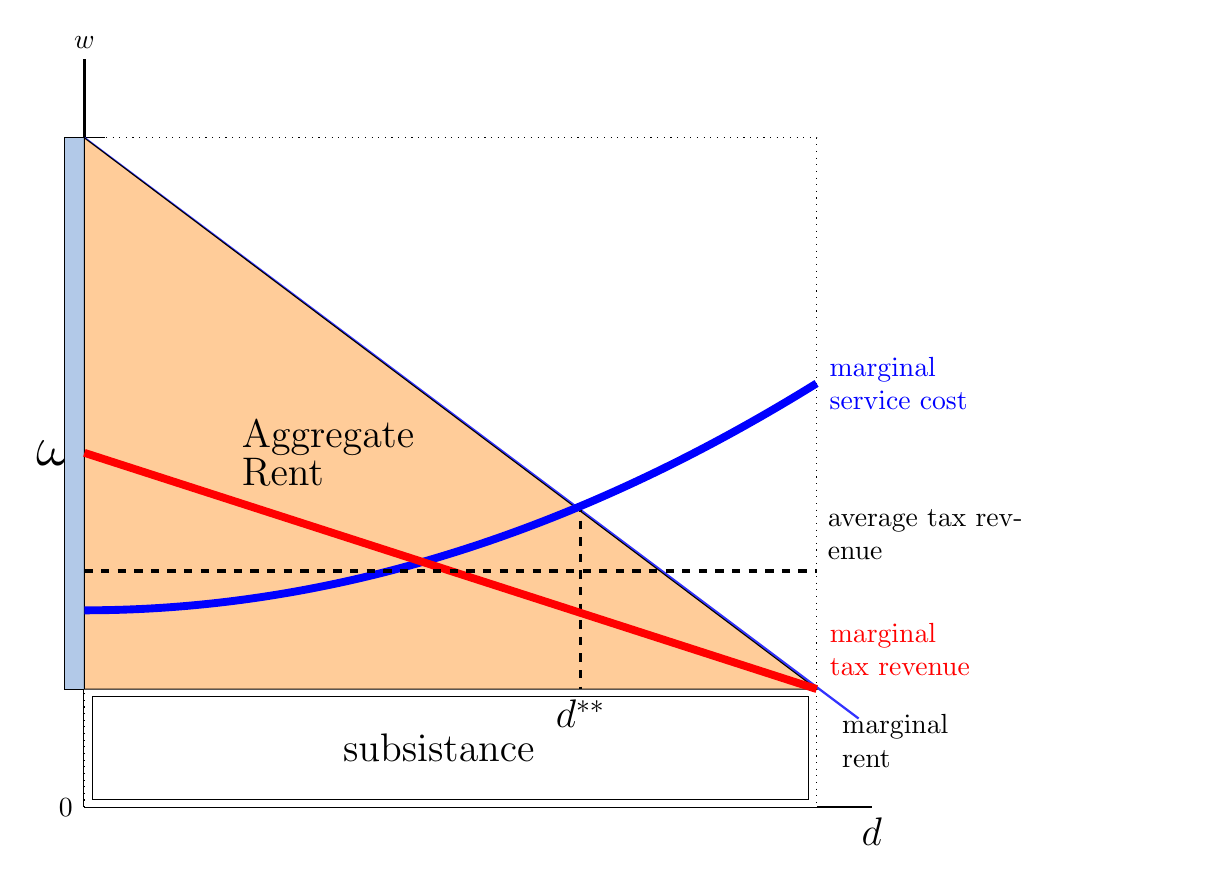
\begin{tikzpicture}[scale=1]
\def\bndmax{5}        %https://tex.stackexchange.com/questions/68462/filling-a-complex-region-with-tikz
\def\bndmin{0.2}
\def \n {8}  % height of y axis
\def \d {10}  % length  of x axis
\def \t {.75}  %  cost of transportation per unit x
\def \th {1}   %
\def \w {7}    %  wage premium
\def \om{1.5}%  omega =rural wage Zero for urban population
\def \azero{2}
\def \aprime {-.0}	
\tikzset{func/.style={thick,color=blue!80}}	
\draw [thick] (0,-\om) --(\d,-\om)node[below]{\Large$d$};  			% Zero for rural population
\draw [thick] (0,-\om)node[left=.5]{$0$} --(0,\n)node[above]{$w$};	% Y axis

%\draw [thick] (0,0)node[left=.5]{ subsistance}--(\d,0);
\node[left=.25] at (0,3){\huge $\omega$};
%\node[left=.25] at (0,\w+.3){subsistence plus};
%\node[left=.25] at (0,\w-.4){wage premium};	

\draw[fill=white, white] (0.1,-0.1) rectangle (14,-\om+.1);
\draw [fill=green!30!blue!30] (-.25, 0) rectangle(.25, \w);
\node[right] at  (.25, \w/2){Added Productivity};
%\draw [ thick, ->](11.3,-\om/2)--(13, -\om/2)node [right] {\Large $d$};
\draw[fill=blue!40] (0.1,-0.1) rectangle (9.2,-\om+.1);

\draw[fill=black!0, dotted] (0,-\om) rectangle (9.30,\w);% new product repeat
\draw[func, domain=0:\w/\t+.5] plot [samples=200] (\x,{\w-\t*\x}); %rent profile
\draw[fill=blue!0] (0.1,-0.1) rectangle (9.2,-\om+.1);
\node at (4.5,-\om/2){\Large subsistance};
\draw[fill=orange!40,] (0.,0.) -- (0,7)--(9.30,0.)--cycle;% Rent \w-.2
\node[text width=2cm] at (3.,3){\Large Aggregate \\Rent}; 		%Rent 
%\node at (5.8,5.7)[]{\Large Transportation};
\node at (6.3,4.8)[white]{\Large expenditure};
\draw[ line width=.5mm, dashed] (6.3,2.35)--(6.3,0)node[below ]{\Large$d^{**}$};

\draw[func, domain=0:9.3, line width=1mm,blue, text width=2cm] plot [samples=200] (\x,{1+\x^2/30})node[right]{marginal\\ service cost};
\draw[ line width=1mm, red] (0,3)--(9.3,0)node[above right, text width=3cm ]{marginal\\tax revenue};
\node at (9.5, -.2)[below right, text width=2cm]{marginal rent};

\draw[ line width=.5mm, dashed] (0,1.5)--(9.3,1.5)node[above right, text width=2.5cm ]{average tax revenue};

%GRID
%\draw[step=1cm,gray,very thin] (0,0) grid (10,10);

 \end{tikzpicture}

Two stylized facts should be noticed. The first is that the marginal cost of servicing generally  rises with the distance from the centre.  Figure
%~\ref{}
illustrates the general form of servicing costs, but not  the relative scales of rent and servicing costs. When this observation is combined with the `Henry George Theorem" () the conclusion is that the optimal size of the city  is at  $d^{**}$, where marginal service cost intersects with the marginal increase in total urban rent. 

The second stylized fact  is that property taxes, which are generally  fixed as a share of property value, decline as the distance from the centre increases. Figure %~\ref{} 
illustrates the general form of tax liabilities, although it does not  accurately represent their relationship to rent or  servicing costs.  This implies that in many or most urban situations the residents at the outer edges pay less than the average amount in property tax per unit of land, but cost  the community budget more than the average amount. In essence, the central city subsidizes the suburbs. (ref Perverse Cities)
This arrangement is both economically inefficient and unfair, but it has been built into the fiscal structure of cities largely as a result of automobile-based urban growth. It is likely that this fiscal misallocation saps some of the potential productivity growth of cities.

Property taxation reduces the market value of properties, but it also funds services and amenities that increase the value of properties. 

Both servicing and taxation effects are more variable and than the simple model suggests.  One  conclusion urban theorists draw based on variants of the Alonzo model is that because property owners in the low-density urban margin are subsidized,  the subsidy is likely to create serious fiscal problems for municipalities in the long term and result in serious inefficiency in land use. 



\section{Implications and results from Alonzo's  model}
Even with its brutal (or elegant) simplifications, the simple model  can  describe  many features of urban structure and urban history. In this section, we illustrate some of the insights supported by the model. Extensions can incorporate variations in wages, density, transportation costs,  preference, and even building technology and codes. The limitations of the simple, continuous, equilibrium-based versions described above can be overcome using agent-based models to model the evolution of complex and much more realistic urban systems. 



\subsection{Adding Jacobs-style agglomeration effects}
A device in this thesis is to focus on the urban wage premium that attracts workers to the city and pays their living and transportation costs. As we have argued above, there is a premium because of a variety of agglomeration effects that we do not specify that make urban labor more productive than non-urban labour. The process has very deep historical roots and we do not need to provide an origin story for our project. We do need to emphasize the self-reinforcing nature of the mechanism.

An increase in the productivity due to the various spillover effects discussed in the literature eventually is passed through, at least in part, to the wage. Conventional microeconomic theory can be brought to bear to provide a rough sketch the  complex process, which is generally slow, variable, and may involve many unsynchronized lags.  tghe basic process is thgat a firm, discovering its workers are  more productive than expected, enjoys unexpected output and profits. Since the marginal product of each worker is higher that expected, the firm  wants to hire more workers. To do so in a city with full employment, it must raise its wage offer. The increased wage attracts workers from other firms, putting pressure on them to also increase their wage. Wages rise across the city. The general increase in the wage attracts more workers to the city. 

The increase in wages appears at first as a benefit to workers as workers. The area in blue-green represents the worker's share of the increased productivity of the city. The increase is also translated with further lags into rising home prices across the city and rising rental prices for tenants. 

% CHANGING WAGE PREMIUM

\begin{center}
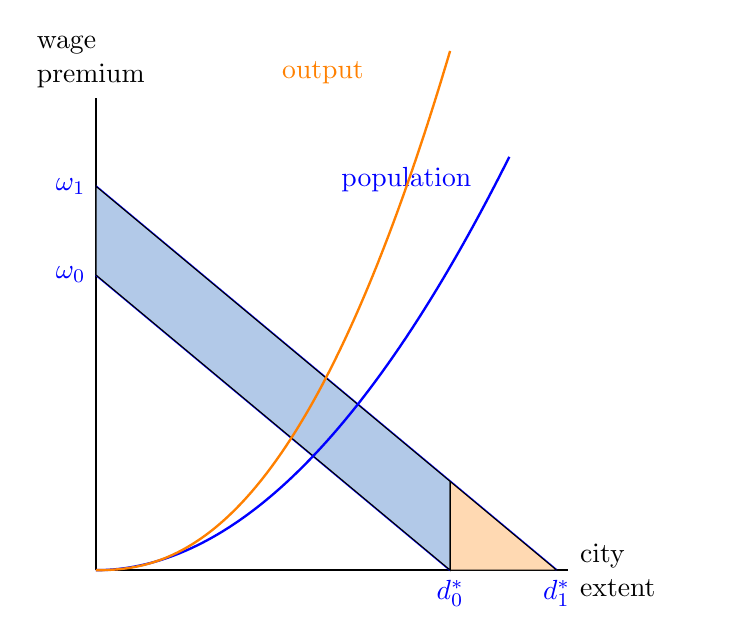
\begin{tikzpicture}[scale=.75]
\def\bndmax{8} 
\tikzset{func/.style={color=blue!80}}	
% EXTENT  BEFORE
\draw[thick](0,0)--(0,8)node[above, text width=1.5cm]{wage \newline premium}; % Y axis
\draw[thick](0,0)--(8,0)node[right=.5, text width=1.5cm]{city\newline extent};  % X axis
%\node at (3.5,-.7){Extent: Walkers};
\draw[thick, blue](0,5)node[left]{$\omega_0$}--(6,0)node[below]{$d^*_0$};
\draw[ thick, blue](0,{5*1.3})node[left]{$\omega_1$}--({6*1.3},0)node[below]{$d^*_1$};
\draw[fill=green!30!blue!30](0,5)--(0,{5*1.3})--(6,5*0.3)--(6,0)--cycle;
\draw[fill=orange!30]({6*1.3},0)--(6,5*0.3)--(6,0)--cycle;
\draw[func, domain=0:7, line width=.3mm,blue, text width=2cm] plot [samples=200] (\x,{\x^2/7})node[below left]{population};
\draw[func,  domain=0:6, line width=.3mm, orange, text width=2cm] plot [samples=200] (\x,{\x^2.3/7})node[below left]{output};
%\node[circle,draw=black, fill=white, inner sep=3pt,minimum size=10pt] (b) at (1,2.5) {1};
\end{tikzpicture}
\end{center}

Assuming that marginal and use per new resident is constant, city size will eventually increase in proportion to the increase in the wage, shown as the distance $d^*_0--d^*_1$. Aggregate rent  further expands by the area shown in orange. Population increases in proportion to the square of the increase in the wage, as illustrated with the blue line.  Output increases super-linearly with population, illustrated by the orange line. 

Adding to the  housing stock is a slow process, introducing potentially complex stock/stock-price dynamics.

The increase in population well eventually generate additional agglomeration benefits, further increasing wages. At the aggregate level this positive feedback appears to be solidly supported, but locally, within firms and between firms there will be long and variable lags. Analytical equilibrium models seek to bypass these messy processes, while agent-based models attempt to incorporate them.

\subsection{Differential transportation costs}
 Urbanists agree that before the railroad and the automobile, the extent of a city was roughly determined by how far a person could walk in about an hour. The time and effort cost of transportation determined the size of cities. 
 
 It also affected the distribution of the classes within the city. When everyone walked, the  wealthy may have valued their time more than the poor. In terms of the model, the willingness to pay for the rich would begin higher than it would for the poor, but would descend more rapidly with distance

\begin{center}
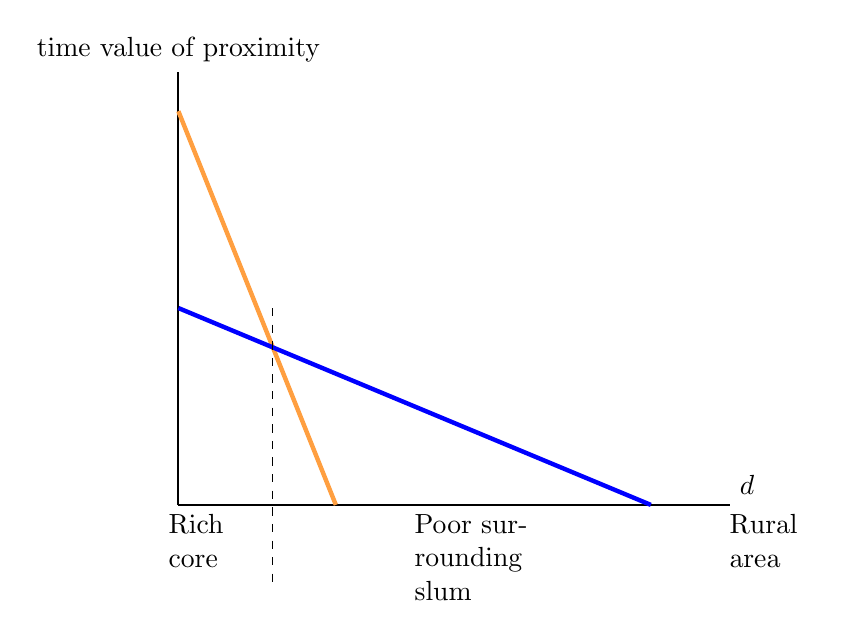
\begin{tikzpicture}[scale=1]

    \draw[thick](0,0)--(0,5.5)node[above]{time  value of proximity}; %Y
\draw[thick](0,0)--(7,0)node[above right]{$d$}; %X

\draw[ultra thick, orange!75](0,5)--(2,0);
\draw[ultra thick, blue](0,2.5)--(6,0);
% \node[draw=white, fill=white] (b) at (1,2.9) {Rich};
% \node[draw=white, fill=white] (b) at (3,1.25) {Poor};
\draw[dashed](1.2,2.5)--(1.2,-1) ;
\node[text width =1cm, below left] at (1,0){Rich core};
\node[below, text width =2cm] at (4,0){Poor surrounding slum};
\node[below, text width =1cm] at (7.5,0){Rural area};
% \draw[ blue, dashed](0,5)--(15,2.5);
% \node[circle,draw=black, fill=white, inner sep=3pt,minimum size=10pt] (b) at (7,3.75) {3};

% \draw[ blue, dotted](0,6.75)--(15,4.25);
% \node[circle,draw=black, dotted,fill=white, inner sep=3pt,minimum size=10pt] (b) at (7,5.5) {4};

 \end{tikzpicture}\end{center}

 If the technology suddenly provides the rich with commuter trains or automobiles and more attractive sites at the edge of the city, the orange line could drop enough  and become much flatter leading in a flight of the rich to the suburbs, as appears to have happened in many American cities. Lower transportation costs make cheaper land on the 

\subsection {Changing transportation costs}

Another application of the model is to the effect of a transportation revolution. The advent of first rail transportation and then the automobile radically changed the size, productivity, and population distribution of cities.
periphery available, allowing larger lot sizes and larger homes for those who can afford them.

% CHANGING TRANSPORTATION COSTS
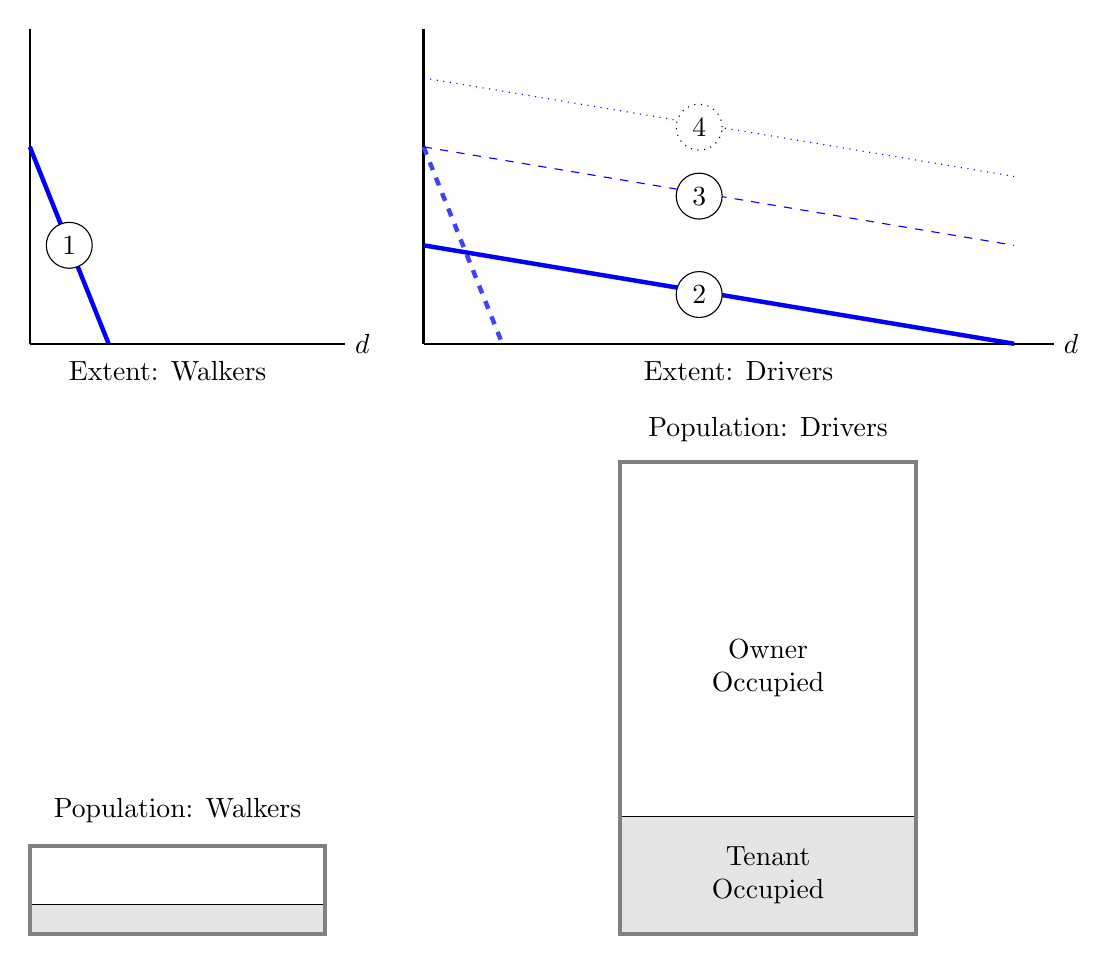
\begin{tikzpicture}[scale=.5]
% EXTENT  BEFORE
\draw[thick](0,0)--(0,8); %Y
\draw[thick](0,0)--(8,0)node[right]{$d$};
\node at (3.5,-.7){Extent: Walkers};
\draw[ultra thick, blue](0,5)--(2,0); 
\node[circle,draw=black, fill=white, inner sep=3pt,minimum size=10pt] (b) at (1,2.5) {1};

% POPULATION BEFORE
\begin{scope}[shift={(0, -15cm)},scale=1.5]%population
\draw [fill=gray!20,] (0,0) rectangle (5,.5); 
\draw[line width= .5mm, black!50] (0,0) rectangle (5,1.5);
\node at (2.5,2.1){Population: Walkers};
\end{scope}

% EXTENT AFTER
\begin{scope}[shift={(10cm, 0)}]
\draw[thick](0,0)--(0,8); %Y
\draw[thick](0,0)--(16,0)node[right]{$d$}; %X
\node at (8,-.7){Extent: Drivers};
\draw[ultra thick, blue!75, dashed](0,5)--(2,0);
\draw[ultra thick, blue](0,2.5)--(15,0);

\node[circle,draw=black, fill=white, inner sep=3pt,minimum size=10pt] (b) at (7,1.25) {2};

\draw[ blue, dashed](0,5)--(15,2.5);
\node[circle,draw=black, fill=white, inner sep=3pt,minimum size=10pt] (b) at (7,3.75) {3};

\draw[ blue, dotted](0,6.75)--(15,4.25);
\node[circle,draw=black, dotted,fill=white, inner sep=3pt,minimum size=10pt] (b) at (7,5.5) {4};
\end{scope}

% POPULATION AFTER
\begin{scope}[shift={(15, -15cm)},scale=1.5]%population
\draw [fill=gray!20,] (0,0) rectangle (5,2); 
\draw[line width= .5mm, black!50] (0,0) rectangle (5,8);
\node at (2.5,8.55){Population: Drivers};
\node at (2.5,4.5)
    [text width=2.4cm, align=center]
    {\baselineskip=20pt Owner Occupied};
%\node at (2,3.3)    [text width=2.4cm]    {\baselineskip=20pt Mortgaged};
\node at (2.5,1)
    [text width=2.4cm, align=center]
    {\baselineskip=20pt Tenant Occupied};
\end{scope}
\label{fig-rent-driving}
 \end{tikzpicture}
 
%\input{fig_TransportCost.tex}

The transportation cost revolution brought about by the first street cars and later automobiles made much larger cities possible.  The average walking pace is 2.5 to 4 mph, and new transportation technologies raise this rate by a factor of between five and ten, increasing potential urban area by between twenty-five and one hundred times.   

% THIS IS INTERSTING K.  morgages: Effect of a finbancial instument on urban form!!  suburban flight, second half of the century

%Electric trolleys drew upon manufacturing technology that appeared only in the eighteen eighties and at first only in America. 

%As with other transportation revolutions, institutional as well as technological revolutions were necessary for the interurban phenomenon to succeed.  One such institutional revolution was the creation of the home mortgage in the eighteen eighties.  Another was the development of the public utility, a regulated monopoly, in the earlier twentieth. century.\footnote{https://faculty.washington.edu/jbs/itrans/charge20.htm} The automotive revolution was as important in its way as the coming of the railroads.

%The automobile in time established even more powerful synergies, but they weren’t present at the beginning.  Roads suitable for automobiles scarcely existed though new methods of paving utilizing macadam or concrete had recently been invented.  Furthermore, there was no good model in place for road construction.   Unlike the case with either light or heavy rail systems, the vehicles and the road itself were not part of the same corporate entity.       

%Once automotive ownership assumed certain proportions toward the close of the teens of the century, the automobile began to transform the landscape of America in an even more fundamental way than the streetcars had. 

%From the second decade of the twentieth century, the automobile in America has been linked with suburban flight, and when the growth of suburbs reached a crescendo early in the second half of the century, automobile ownership became the norm. 

% Because exurbs are already numerous and growing more so, they place considerable pressure on the Body Politic to ensure that fuel prices remain low, for if prices rise beyond a certain point the exurbanites will be forced to sell out, probably at ruinously low returns because few will choose to live in isolated areas without affordable transportation.  True, exurbs could conceivably be served by public transportation, but only at enormous cost per rider because the population densities are so low in the areas where they are located....

% That places the vast suburb dwelling public at risk and the exurbanites most of all.

Initially, rents fell at the centre and rose outside of the original city limits. Lower rents and cheaper suburban housing attract more workers, so that central rents and the land values they support  rise to the original levels and then, because the rising population makes the city more productive, beyond the original level. 

It  also affected social structure and left indelible marks on the form of cities developing at the time and after. In North America, with large amounts of land, it generated massive urban sprawl, but also made land available for a growing `middle class' of homeowners. This homeowning middle class became the dominant social formation in North 
American society. 

Ultimately the urban expansion generated congestion and rising transportation cost that began to limit urban growth, put upward pressure on  housing costs including transportation, and therefore downward pressure on middle-class effective incomes. Rising congestion costs steepen the rent profile and  reduce the net productivity of cities. Although the process is not a focus of this thesis it represents a relatively simple extension for later work.



\subsection{Class structure}\label{sec-class-structure}

At the stage illustrated on the right  in Figure~\ref{fig-rent-driving},  %(Alonzo city suburbanized with owner occupiers) 
as a result of rapidly rising productivity, falling transportation costs, and large amounts of land with relatively low productivity, a new urban social system has emerged with a land-owning working class. This is a recent phenomenon, and perhaps primarily a North American one. We are concerned in this thesis with whether it is also also be a passing stage.

America's economic transformation in the early 1800s was linked to dramatic changes in transportation networks. Construction of roads, canals, and railroads led to the expansion of markets, facilitated the movement of peoples, and altered the physical landscape. The later commuter transportation revolution  further transformed cities and class structures.

\begin{center}
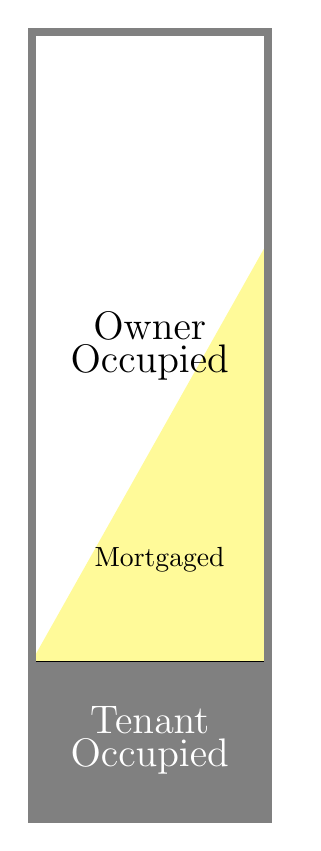
\begin{tikzpicture}{scale=.5}
\draw [fill=gray,] (0,0) rectangle (3,2); %TENANT
\draw [fill=yellow!40] (0,2)--(3,2)--(3,7.33); --cycle;% MORTGAGE %Calculation. 80\%owner, so  8 above the tenant line. 2/3*8=5.333. 5.333+2=
\draw[line width= 1mm, black!50] (0,0) rectangle (3,10);
\node at (1.5,6)
    [text width=2.4cm, align=center]
    {\baselineskip=20pt\Large Owner Occupied};
\node at (2,3.3)
    [text width=2.4cm]
    {\baselineskip=20pt Mortgaged};
\node at (1.5,1)
    [text width=2.4cm, align=center, white]
    {\baselineskip=20pt\Large Tenant Occupied};
\end{tikzpicture}

Figure: Housing Tenure post transportation revolution
\end{center}

Belderbos et. al examine the simultaneous effects of spillovers due to research and development by universities and by firms \cite{belderbosWhatSpilloversUniversities2022}. Rising urban productivity in Japan are significant. 

%will raise the wage, attracting more workers. If they are added in suburbs at the edge of the city (Ricardo's extensive margin) virtually all of the wage premium they receive is dissipated in transportation costs. Closer to the centre,  land rents rise. Owner-occupiers capture the increase as property value appreciation. Tenants are likely to be faced with higher rents.      

%If agglomeration is the source of productivity gains, however, the new workers increase the urban premium, further increasing land values and attracting more workers. 

%The rural population consists of uniformly distributed efficient mix of rural capital producers and workers, all of whom receive $\omega$.%\footnote{This does nothing but fix the price of produced capital in terms of the rural wage.} 

 %Owners of urban firms are  conventional  capitalists, who may earn excess profit if they can capture an unearned surplus from labour.  Any unearned surplus increases the return to urban capital relative to rural capital, resulting in continual expansion of the urban economy. Continuous growth in turn results in continuously rising urban land prices and hence housing costs. We ignore the distributional implications of this feature of the model, and focus instead on the part of value produced by the city that appears as land rent. 

In this chapter we have described a very abstract, stylized model to establish how land rents are generated in the urban system and how they are related to neoclassical growth theory. One feature of this model is that none of the simplifying assumptions are essential. The mode can easily be generalized in many ways. We maintain the basic simplicity but..  


\section{Notes}
Maybe add reference to central place theory. % \gls{central place} \gls{central place theory}